\documentclass[10pt,a4paper,DIV14]{scrartcl}
%\usepackage{german}
\usepackage{umlaut}
\usepackage{longtable}
\usepackage{fancyvrb}
\usepackage{makeidx,rotating,graphicx,array}

\pagestyle{myheadings}
\markright{\today}
\begin{document}

\centerline{\Large \bf Assignment 1}
\vspace{5mm}
\centerline{\Large  SQL}
\vspace{12mm}

% createdb <name>
% psql <name> -e < course_dump
Load the {\it course\_dump} to a new database. give an
systemewide unique name for the database.
\vspace{5mm}

The structure of the database are shown in figure \ref{stru}.
\vspace{5mm}

% \d
% \d animal
% \da
% \h update
{\bf psql:}
\begin{enumerate}
\item list all tables
\item list all columns for table animal
\item list all users
\item get help on sql command update
\end{enumerate}


% psql \d...
% select * from station limit 10
% select db_animal, db_breed, db_sex, birth_dt from animal limit 10
% select ext_animal, ext_breed, ext_sex, birth_dt from v_animal limit 10
% select distinct ext_animal, ext_breed, ext_sex, birth_dt from v_animal limit 10
% select distinct ext_animal, ext_breed, ext_sex, birth_dt from
%     v_animal where ext_breed notnull limit 10
% select ext_breed from v_animal group by ext_breed
% select ext_breed, count(*) from v_animal group by ext_breed
% select db_animal, min(born_alive_no), avg(born_alive_no), max(born_alive_no), count(born_alive_no) from litter group by db_animal having count(born_alive_no) > 1 order by avg(born_alive_no) desc;
{\bf SELECT:} use allways an limit option at the end!
\begin{enumerate}
\item show all components from table STATION
\item display db\_animal, db\_breed, db\_sex, birth\_dt from table
  ANIMAL
  \begin{enumerate}
%  \item show the external representations of it
  \item only if breed exist
  \item order by birth\_dt
  \end{enumerate}
\item show each dam only one time
% \item only animal 'society$|$sex:::32$|$2:::111772' (use like)
\end{enumerate}

\begin{figure}[htb]
   \centering  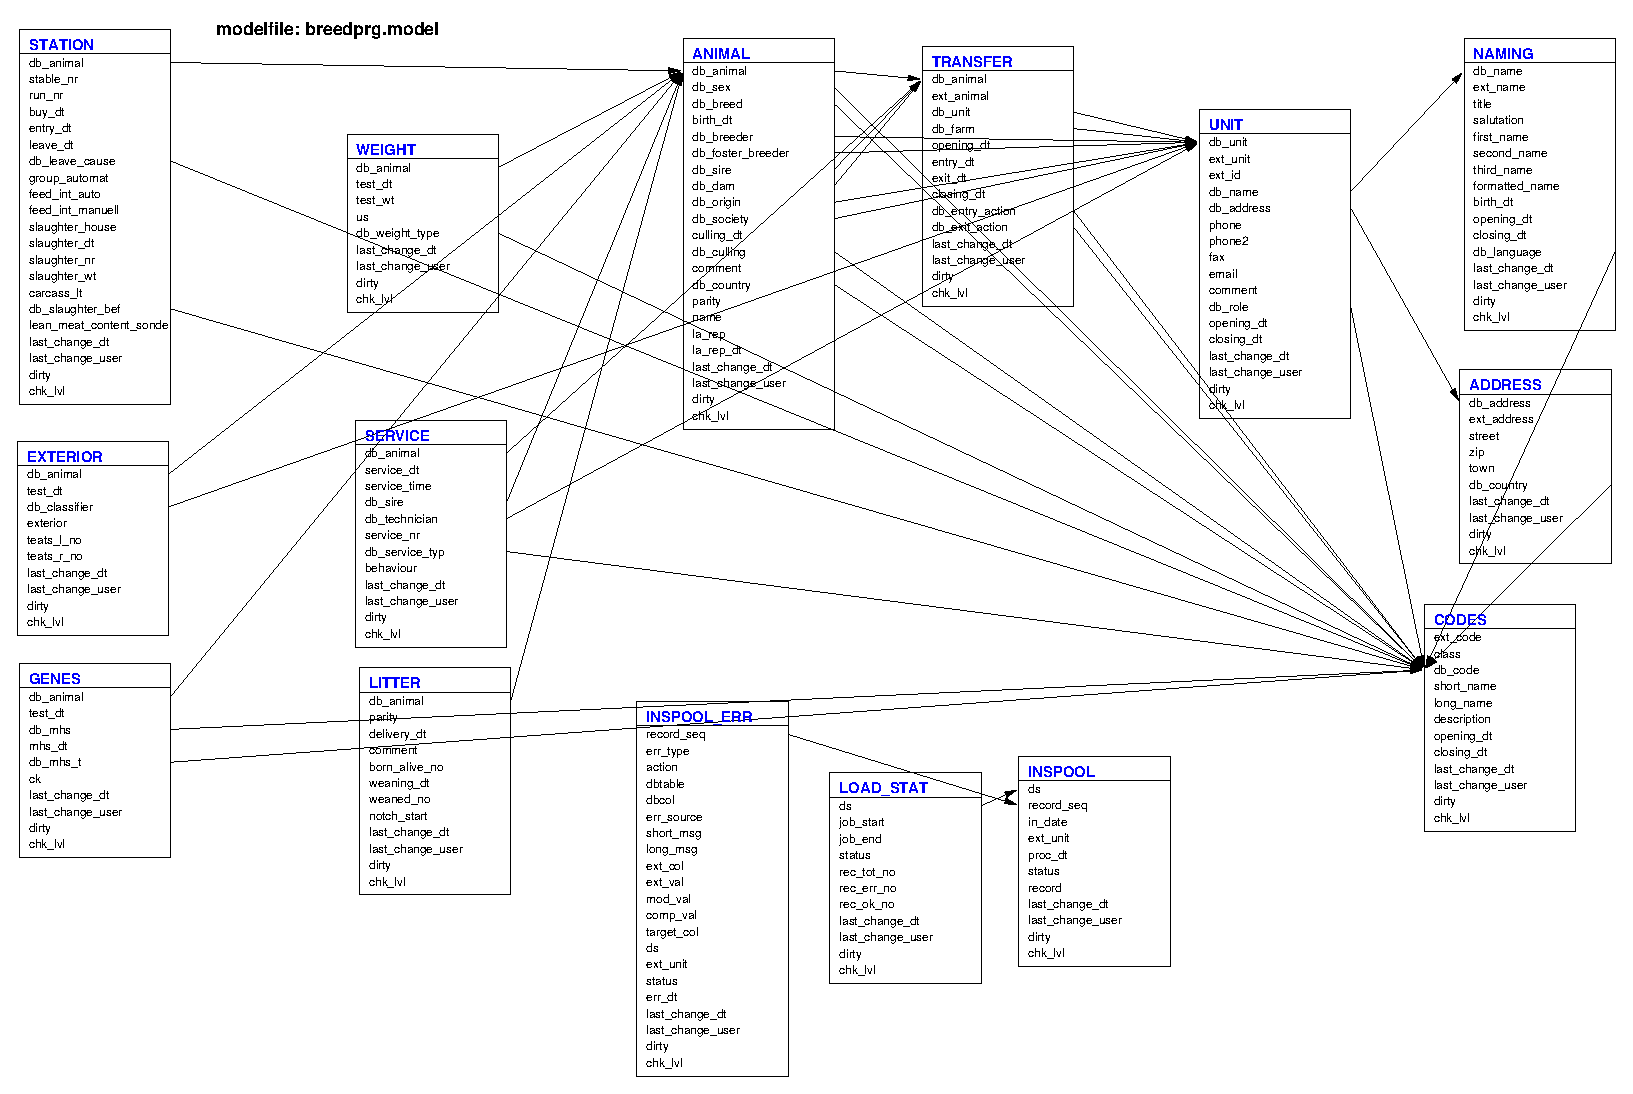
\includegraphics[scale=0.9, angle=90]{breedprg.model.eps}
   \caption{Table Structure}
\label{stru}
\end{figure}



\newpage

\centerline{\Large \bf Assignment 2}
\vspace{5mm}
\centerline{\Large  SQL}
\vspace{12mm}

\begin{enumerate}
\item {\bf SELECT}
\begin{enumerate}
\item show the number of records in table litter and table service
\item show the number of animals in table litter and service
\item list all different society
\item count the number of animals for each society
\item display minimum, average and maximum litter size for each animal
  \begin{enumerate}
  \item add the count
  \item sort the display by the average descending
  \item display only if there more than one record
  \end{enumerate}
\item get the db\_breed for breed DL (this means external code in
  table codes)
\item get all animals where breed is DL
\item add the longname and description for db\_breed from table codes
% select a.db_animal, b.db_mhs from animal as a, genes as b where a.db_animal = b.db_animal and a.db_breed = 36;
\item get all DL animals which have an mhs genotype
% select a.db_breed, count(b.db_mhs) from animal as a, genes as b where a.db_animal = b.db_animal group by a.db_breed;
  \begin{enumerate}
% select a.db_animal, b.db_mhs, birth_dt from animal as a, genes as b where a.db_animal = b.db_animal and a.db_breed = 36 and birth_dt > '01-01-1998' order by birth_dt desc ;
  \item add the birth date to these animals 
  \item order by birth date
  \item display only if are born after 1998
  \end{enumerate}
\item count these animals
\end{enumerate}

% select * from codes where class = 'WEIGHT_TYPE'
% insert into weight (db_animal, test_dt, test_wt, db_weight_type ) values ( 143, '12-12-2004', 127, 5 )
\item {\bf INSERT:}
\begin{enumerate}
\item get an existing internal weight type ('FIELD')
\item insert n
ew record in table WEIGHT (internal db\_animal = 143,
  date = today, weight = 101, weight type = 'FIELD' )
\end{enumerate}

% select db_animal from v_animal where ext_animal like '%2:::130192'; 
% select * from codes where ext_code = 'PI';
% update animal set db_breed = 56 where db_animal = 11;
\item {\bf UPDATE:}
\begin{enumerate}
\item update breed to PI for animal society$|$sex:::32$|$2:::130192 (get
  first the internal numbers and update then)
\end{enumerate}
\end{enumerate}

%\newpage

%\centerline{\Large \bf Assignment 3}
%\vspace{5mm}
%\centerline{\Large  SQL}
%\vspace{12mm}


\end{document}

